% Asado a la cacerola
\newpage
%\thispagestyle{empty}
\begin{recipe}[source={El papá},
portion={4-6 porciones},
preparationtime={\unit[2]{Horas}}
]{Asado A La Cacerola}
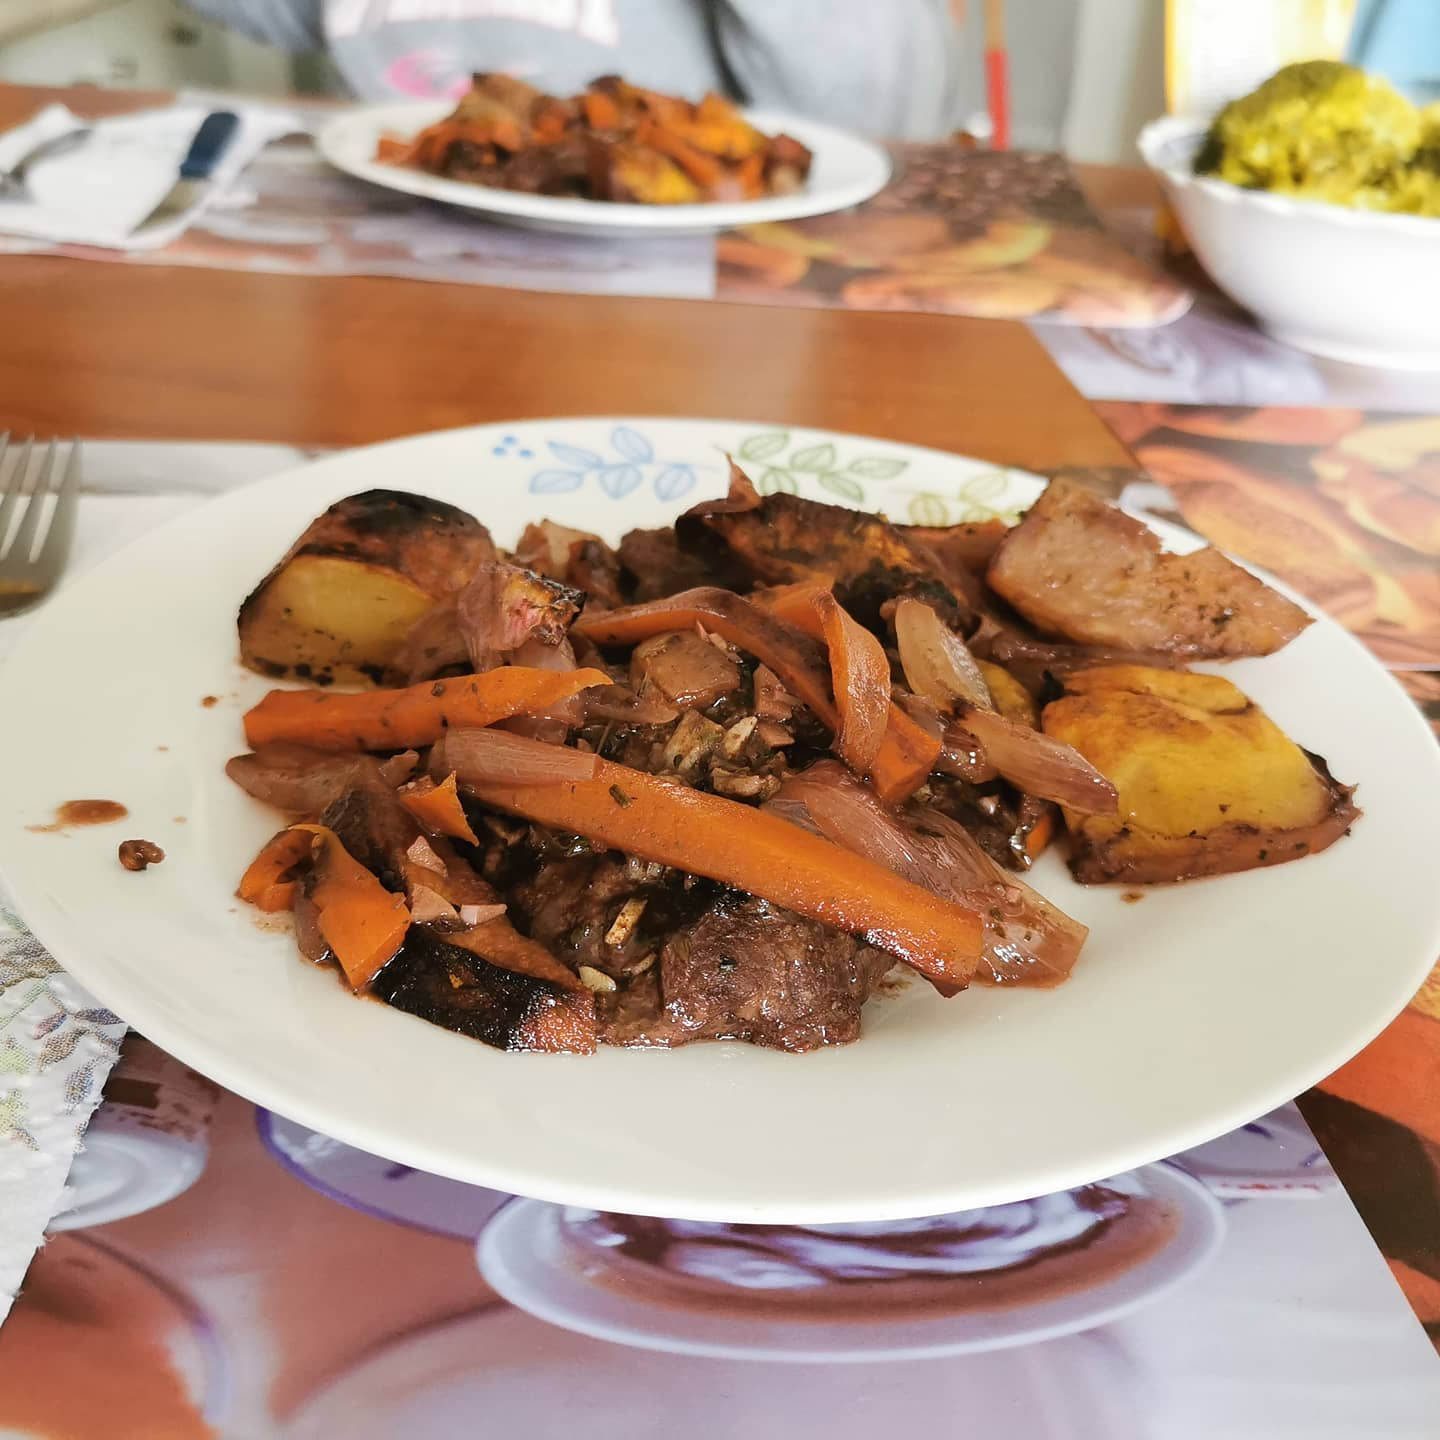
\includegraphics[width=0.25\textwidth]{asado-cacerola}
\introduction{
Esta es una receta muy añorada por mi familia. Era una de las especialidades de mi padre.
}
\ingredients{
    \unit[2]{Kg} & de carne de punta ganso \\
    2 & Cebollas cortadas en 4 \\
    2 & Manzanas cortadas en 4 \\
    3 & dientes de ajo picados \\
    & Orégano a gusto \\
    5 & papas \\
    2 & zanahorias cortadas en tiras finas a lo largo \\
    \unit[150]{gr} & Vinagre \\
    1 & copa de vino tinto \\
      & Aceite de oliva \\
      & Sal \\
      & Pimienta
}
\preparation{
    \begin{enumerate}
        \item Adobar la carne con los aliños y dejarla macerar al menos media hora como mínimo.
        \item Pre calentar el horno a 180 grados por 5 minutos.
        \item En una fuente para horno, meter la carne adobada con los aliños, la cebolla, la manzana, la zanahoria, las papas y finalmente la copa de vino.
        \item Meter la bandeja al horno y dejar cocinar por aproximadamente 2 horas.
        \item Retirar y servir. 
    \end{enumerate}
}
\hint{
	Se puede acompañar con arroz o ensalada.
}
\end{recipe}